\documentclass{standalone}
\usepackage{tikz}

\newcounter{node}

\begin{document}
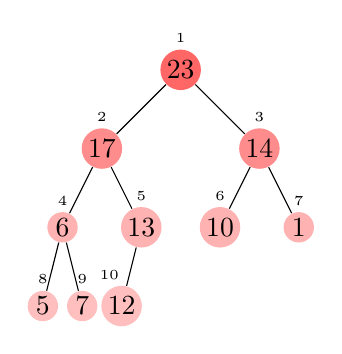
\begin{tikzpicture}
  [level distance=10mm,
    every node/.style={fill=red!60,circle,inner sep=1pt},
    level 1/.style={sibling distance=20mm,nodes={fill=red!45}},
    level 2/.style={sibling distance=10mm,nodes={fill=red!30}},
  level 3/.style={sibling distance=5mm,nodes={fill=red!25}},
]
  \node[label={90:\tiny1}] {23}
  child {node[label={90:\tiny2}] {17}
    child {node[label={90:\tiny4}] {6}
      child {node[label={90:\tiny8}] {5}}
      child {node[label={90:\tiny9}] {7}}
    }
    child {node[label={90:\tiny5}] {13}
      child {node[label={95:\tiny10}] {12}}
      child[missing]
    }
  }
  child {node[label={90:\tiny3}] {14}
    child {node[label={90:\tiny6}] {10}
      child [missing]
    child [missing]
    }
    child {node[label={90:\tiny7}] {1}
        child [missing]
        child [missing]
    }
  };
\end{tikzpicture}
\end{document}





